%%%%%%%%%%%%%%%%%%%%%%%%%%%%%%%%%%%%%%%%%%%%%%%%%%%%%%%%%%%%%%%%%%%%%%
\paragraph{Summation versus sampling}
%%%%%%%%%%%%%%%%%%%%%%%%%%%%%%%%%%%%%%%%%%%%%%%%%%%%%%%%%%%%%%%%%%%%%%

When calculating the cross section for a given process, an integral
over the relevant phase space has to be performed, typically through
Monte Carlo methods.  Then, for each phase-space point (\ie for each
set of incoming and outgoing momenta) the matrix element squared has
to be evaluated.  This involves a summation and averaging over the
unobserved quantum numbers of the outgoing and incoming particles,
respectively.  On the level of squared amplitudes the summation can be
performed analytically, involving algebraic relations such as
completeness relations or the Dirac trace algebra, which yields an
analytical result for the squared matrix elements, that can in turn be
expressed by Lorentz-invariant combinations of the four-momenta of the
involved particles.  This method is typically applied for matrix
elements of low final-state multiplicity, which are pre-computed and
implemented explicitly in the event generators.  On the level of
numerically evaluated amplitudes, on the other hand, one may choose
between a summation over all quantum states such as helicities and
colours for a given phase-space configuration and a Monte Carlo
sampling over these states, together with the phase-space integration.
The computational complexities for summation and sampling for matrix
elements with $n$ external lines naively differ by the
$n^{\mathrm{th}}$
power of the number of possible states, \ie usually ${\cal
  O}(2^n)$ for the possible helicity assignments and ${\cal
  O}(3^{n_3}8^{n_8})$ for the possible colour assignments of $n_3$
external quarks and $n_8$ external gluons.  By suitably eliminating
common subexpressions of the matrix elements, one can, however, often
reduce these naive factors quite considerably.  The decision whether
to sum or to sample over helicity and colour degrees of freedom is
therefore strongly dependent on the process and the particle
multiplicity.  Corresponding comparisons have been presented, \eg
in~\cite{Gleisberg:2008fv}. This issue will not be discussed further
here.  We will, however, discuss different techniques to efficiently
deal with coloured states, as the sum over colours usually poses the
most severe restriction on the ability to evaluate high-multiplicity
matrix elements.
 
%%%%%%%%%%%%%%%%%%%%%%%%%%%%%%%%%%%%%%%%%%%%%%%%%%%%%%%%%%%%%%%%%%%%%%
\paragraph{Pre-computed matrix elements} 
%%%%%%%%%%%%%%%%%%%%%%%%%%%%%%%%%%%%%%%%%%%%%%%%%%%%%%%%%%%%%%%%%%%%%%

Traditionally, the matrix elements acting as seeds for event generation have
been related to processes with low multiplicity of two or maximally three
particles in the final state.  For such processes, analytical results are
usually available, and consequently they are used in all event generators.
With the advent of multijet merging methods and agreements for interface
structures, the importance of incorporating such matrix elements directly
into MC programs has diminished, such that in the new generation of 
event generators only a few pre-computed analytic matrix elements are available.
On the other hand, due to the incorporation of matching methods for NLO 
matrix elements, some explicit next-to-leading order results are now direct
inputs for event generation, just as leading-order results were previously.
This situation is likely to change, as with the advent of general methods
to automate the computation of NLO virtual corrections the need for explicit
calculations may slowly disappear. 

\paragraph{The helicity method}
%%%%%%%%%%%%%%%%%%%%%%%%%%%%%%%%%%%%%%%%%%%%%%%%%%%%%%%%%%%%%%%%%%%%%%

Textbook methods of squaring full matrix elements and summing over helicity
and colour through the application of completeness relations yields a rather 
large number of terms: for $N$ Feynman diagrams in this method $N(N-1)/2$ contributions
must be evaluated.  An obvious way of reducing this number is to 
directly evaluate the amplitudes, yielding complex numbers, before summing 
and squaring them and before sampling over the phase space.  
In order to compute the individual numerical values of the amplitudes, an 
efficient representation in terms of external momenta and helicities is mandatory.  
A first solution to this problem was achieved in~\cite{Kleiss:1985yh}.  
The basic idea is to replace all momentum-dependent terms appearing
in an amplitude through suitably chosen spinor products. This substitution 
can always be achieved, since spinors are the simplest representations of 
the Lorentz group and their products correspondingly yield the minimal 
representation of a Lorentz-invariant complex number. One can, for example, 
identify the numerator of a fermion propagator as
\begin{equation}
\begin{split}
p\!\!\!/+\mu \;=\; &
\frac12\sum\limits_\lambda
        \left[u(\lambda,p)\bar u(\lambda,p)\;
                               \left(1+\frac{\mu}{\sqrt{p^2}}\right)+
             v(\lambda,p)\bar v(\lambda,p)\;
                              \left(1-\frac{\mu}{\sqrt{p^2}}\right)\right]\;,
\end{split}
\end{equation}
and the polarization vector of a spin-1 boson with momentum $p+q$ can be 
written as
\begin{equation}
\begin{split}
\epsilon_\mu(p+q) \;=\; & \frac{1}{\sqrt{4p\cdot q}}
             \bar u(\lambda,q)\gamma_\mu u(\lambda,p)\,.
\end{split}
\end{equation}
In such a way, and employing a Chisholm identity for terms of the form
$\bar u\gamma^\mu u\times\bar u\gamma_\mu u$, every amplitude containing
fermion interactions can be decomposed into spinor products of the form 
$\bar uu$ and $\bar vv$, see~\cite{Kleiss:1985yh,Ballestrero:1992ed,
  Ballestrero:1992dv,Ballestrero:1994ti}.  
In the context of tree-level matrix-element generators, the corresponding 
elementary building blocks are usually referred to as Lorentz functions.
They are implemented in a similar form in any of the automated 
matrix-element generators listed above.

 
%%%%%%%%%%%%%%%%%%%%%%%%%%%%%%%%%%%%%%%%%%%%%%%%%%%%%%%%%%%%%%%%%%%%%%
\paragraph{Feynman-diagram based methods}
%%%%%%%%%%%%%%%%%%%%%%%%%%%%%%%%%%%%%%%%%%%%%%%%%%%%%%%%%%%%%%%%%%%%%%

Having at hand the basic Lorentz functions to decompose amplitudes into terms that can
be evaluated numerically in a straightforward manner, the remaining problem is
the generation of these amplitudes.  Traditionally this is achieved through
the construction of Feynman diagrams -- an algorithm with improved efficiency using 
recursive relations will be discussed later.  The diagrammatic approach has been followed 
for instance in \Madgraph~\cite{Stelzer:1994ta} and \Amegic~\cite{Krauss:2001iv}.  
In both programs, Feynman-diagram-like topologies, i.e\ trees with binary or tertiary 
vertices, are generated and then filled with the actual interactions given by the physics
model in question.  The resulting objects are translated into so-called helicity amplitudes,
\ie into products of the Lorentz functions discussed in the previous
paragraph.  In so doing, some manipulations may be performed, trying to
identify common subexpressions and either factoring them out or storing them 
such that identical pieces need to be calculated only once.
In both cases, the programs write out the helicity amplitudes in a high-level
programming language to be compiled and linked to the original program. The resulting
libraries are then employed to calculate cross sections, to generate parton-level events
and to pass these events on to a parton-shower simulation, for instance, using Les Houches 
Event Files, see \AppRef{sec:MEinterfaces}.

 
%%%%%%%%%%%%%%%%%%%%%%%%%%%%%%%%%%%%%%%%%%%%%%%%%%%%%%%%%%%%%%%%%%%%%%
\paragraph{Skeletons}
%%%%%%%%%%%%%%%%%%%%%%%%%%%%%%%%%%%%%%%%%%%%%%%%%%%%%%%%%%%%%%%%%%%%%%

In \Herwigpp only a few pre-computed squared matrix elements are 
available.  The authors of this code have, however, compensated for this by 
a low-level matrix-element generator, which is capable of constructing
helicity amplitudes for processes with up to four external particles (\ie
$2\to2$ scattering and $1\to3$ decay processes).  Depending on the spin 
of those particles, the algorithm identifies all possible topologies
($s$, $t$, and $u$-channel as well as four-point interactions) for the 
process in question, with the corresponding propagators being specified by
the Feynman rules given in an internal format.  These topologies are then
directly mapped onto the respective prefabricated helicity amplitudes.
This algorithm greatly alleviates the task of integrating the cross sections 
efficiently: the knowledge of topologies and propagators allows for a direct 
translation into prefabricated integration channels, forming a multi-channel
integrator, see \AppRef{Sec:PS_ME}. For further details of the 
implementation of this algorithm we refer to~\cite{Gigg:2007cr}.

%%%%%%%%%%%%%%%%%%%%%%%%%%%%%%%%%%%%%%%%%%%%%%%%%%%%%%%%%%%%%%%%%%%%%%
\paragraph{Recursive techniques} 
%%%%%%%%%%%%%%%%%%%%%%%%%%%%%%%%%%%%%%%%%%%%%%%%%%%%%%%%%%%%%%%%%%%%%%
There are several techniques for computing tree-level matrix elements that employ 
different versions of recursive relations. With increasing number of particles 
involved in the scattering they are superior to diagram-based methods,
as they naturally implement an optimal common subexpression elimination.
One such method, which we shall consider as an example of a recursive 
technique in this context, is the Berends-Giele algorithm~\cite{Berends:1987me,
  Berends:1987cv,Kleiss:1988ne,Berends:1988yn,Berends:1989ie}.
It has recently been improved to incorporate an efficient way
to deal with colour~\cite{Duhr:2006iq}, rendering it essentially equivalent 
to the Dyson-Schwinger methods employed for instance in 
\Helac~\cite{Draggiotis:2002hm}, and comparable in efficiency with the 
\ALPHA\ algorithm of~\cite{Caravaglios:1995cd}, implemented in 
\Alpgen~\cite{Mangano:2002ea} and \OmegaCode~\cite{Moretti:2001zz}. 
 
\begin{figure}[t]\begin{center}
  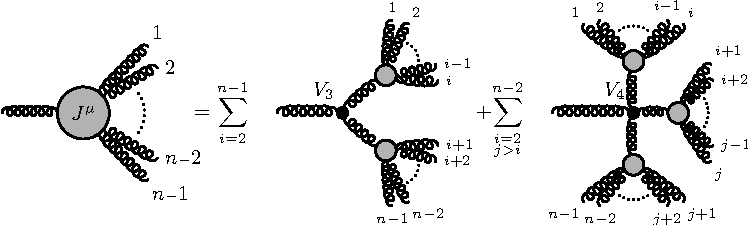
\includegraphics[width=\textwidth]{appendix/matrix-elements/bgrr.pdf}
  \end{center}
  \caption{Pictorial representation of the Berends-Giele 
  recursive relations.\label{fig:BG}}
\end{figure}
The basic idea of the Berends-Giele recursion algorithm can be summarized as 
follows. At first, an $n-1$-point gluon 
off-shell current, $ J^\mu$, is defined, which represents the sum 
of all colour-ordered Feynman diagrams with $n-1$ external on-shell legs 
and a single off-shell leg with polarization $\mu$.  This off-shell current 
can then be decomposed into lower-point off-shell currents, which are joined 
by the elementary gluon interaction vertices, thus forming a bigger part of
the full scattering amplitude. This algorithm is schematically depicted in 
\FigRef{fig:BG}.  A full $n$-gluon amplitude is finally obtained by 
amputating the off-shell propagator and contracting the remaining quantity 
with the external polarization of gluon $n$.  

Similar recursions exist for the off-shell quark currents~\cite{Berends:1987me} 
and for the full Standard Model~\cite{Gleisberg:2008fv}.  They can, in fact, 
be defined for any theory allowing the construction of Feynman diagrams.
A further improvement of this method was recently obtained through a 
decomposition of all four-particle vertices into three-particle ones.
Such a decomposition reduces the computational complexity for
many-particle final states, as the numerical effort grows approximately like 
$N^n$, with $N$ the average number of legs in elementary vertices of the theory.


%%%%%%%%%%%%%%%%%%%%%%%%%%%%%%%%%%%%%%%%%%%%%%%%%%%%%%%%%%%%%%%%%%%%%%
\paragraph{Treatment of colour} 
%%%%%%%%%%%%%%%%%%%%%%%%%%%%%%%%%%%%%%%%%%%%%%%%%%%%%%%%%%%%%%%%%%%%%%

Several methods have been suggested over the past decades to optimize the
computation of amplitudes including QCD particles with respect to the 
colour degrees of freedom.  There are two essentially different approaches:
the textbook method would be to compute colour-ordered quantities, \ie 
sets of Feynman diagrams or off-shell currents with all colour information 
combined into kinematics-independent prefactors.  When assembling the full 
matrix element, colour-factors and kinematics-dependent functions are then
treated separately.  An alternative approach is to directly include colour 
in the diagrams or off-shell currents and to devise, for example, recursive 
relations which depend on the colour quantum numbers.

The latter approach has been very successful in the past, leading to the 
construction of advanced tree-level matrix-element generators, capable of 
dealing with very large final-state multiplicities~\cite{Kanaki:2000ey, 
  Draggiotis:2002hm,Mangano:2002ea,Gleisberg:2008fv}.
The textbook approach, on the other hand, is often much more convenient to use,
especially when insight into the analytical structure of the computation is 
necessary.  It also usually leads to a significant acceleration of 
matrix-element computations for low-multiplicity final states.

Although a number of possible colour bases exist~\cite{Mangano:1987xk,
  DelDuca:1999ha,DelDuca:1999rs}, which have been used for
several numerical comparisons in the past~\cite{Duhr:2006iq}, the 
one that is widely adopted today is the colour-flow 
basis~\cite{Kanaki:2000ey,Maltoni:2002mq}. The reason for its superior 
speed in the computation of large-multiplicity QCD amplitudes lies not only 
in the milder growth in the number of possible colour-ordered amplitudes, but 
also in the fact that every colour coefficient multiplying the 
kinematics-dependent functions in squared matrix elements consists only 
of delta functions, which are trivial to evaluate in a Monte Carlo program.
